% Metaphor: hub-and-spoke network. Everything goes through one place --
% reach for it when *that* is the claim, since it is the shape a reader
% reads a broker, a registry or a single point of failure off.
%
% Idiom: a star. Every spoke is placed relative to the hub, so the hub
% stays the centre of the picture as well as of the argument, and a
% spoke can be added without re-deriving anyone else's coordinate.
\usetikzlibrary{positioning}
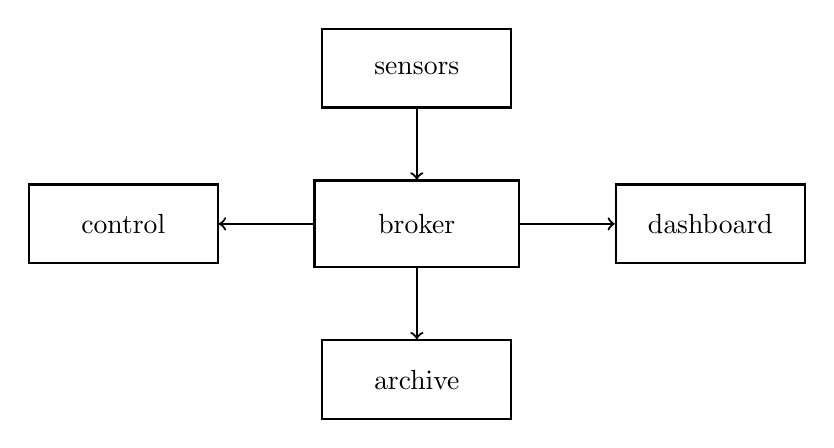
\begin{tikzpicture}[thick,
                    spoke/.style={draw,align=center,
                                  minimum width=24mm,minimum height=10mm},
                    hub/.style={draw,align=center,
                                minimum width=26mm,minimum height=11mm}]
  \node[hub] (broker) {broker};
  \node[spoke,above=9mm of broker] (sensors) {sensors};
  \node[spoke,below=9mm of broker] (archive) {archive};
  \node[spoke,left=12mm of broker] (control) {control};
  \node[spoke,right=12mm of broker] (dashboard) {dashboard};
  \draw[->] (sensors) -- (broker);
  \draw[->] (broker) -- (archive);
  \draw[->] (broker) -- (control);
  \draw[->] (broker) -- (dashboard);
\end{tikzpicture}
